% !TeX program = xelatex
% 编译：xelatex news_views_skeleton.tex（连续运行两次）。
% 这是写作骨架，不是已经完成的 800--1000 词文章。
% 下列十段的英文概括句是每段的起点；请按中文注释自行扩写。
% 正文词数预算：80+70+90+90+100+90+90+90+110+90 = 900 词。
% 预算不包括标题、导语、图注和参考文献；若课程将图注计入，总量仍可压在1000词以内。
% 仿照 Spitz 的 News & Views：首段点题，必要背景，概括方法，结果，评价与展望。
% 不设正文小标题；不讲 KDE 的实现、网络层数、激活函数或损失函数。
% 标题与导语也只是可修改的工作版本。
\documentclass[11pt,a4paper]{article}
\usepackage[margin=24mm]{geometry}
\usepackage{fontspec}
% \setmainfont{Latin Modern Roman}
% \setsansfont{Latin Modern Sans}
\usepackage{amsmath,graphicx,microtype,float}
\usepackage[super,sort&compress]{natbib}
\usepackage{xcolor}
\usepackage[colorlinks=true,urlcolor=blue!55!black,citecolor=blue!55!black]{hyperref}
\usepackage[font=small,labelfont=bf]{caption}
\setlength{\parindent}{1.2em}
\setlength{\parskip}{4pt}
\setlength{\emergencystretch}{2em}
\clubpenalty=10000
\widowpenalty=10000
\raggedbottom
\begin{document}

% \noindent{\sffamily\small NEWS \& VIEWS \quad GRAVITATIONAL-WAVE ASTRONOMY\par}
% \vspace{5pt}
\noindent{\LARGE\bfseries Learning as a shortcut to gravitational-wave inference\par}
\vspace{8pt}
\noindent\textbf{A neural approximation to an expensive likelihood could make
  gravitational wave analysis faster and more adaptable.}
\vspace{8pt}

% P1 | 引入与点题 | 扩写后约80词
% 先写事件数量、波形复杂度和重复分析带来的计算压力，再引入Negri与Samajdar。
% 说明FLEX在既有贝叶斯框架中替换昂贵的似然评估；它不替代贝叶斯推断本身。
% 可预告GW150914特定比较中的约16倍时间加速；不要把调用次数减少百倍当作总时间加速。
% 不加入未经更新核实的“目前已探测多少事件”数字。
% \noindent Extracting the physics from a growing stream of gravitational-wave
% signals is becoming computationally demanding. Negri and Samajdar propose
% learning a fast approximation to a costly step in the analysis.\cite{negri2025}

Gravitational waves (GW) are ripples in spacetime intrigued by movement of massive objects such as black holes or neutron stars. Decade after the first observation of GW plenties of signals are thereafter recorded, meanwhile more complicated theoretical models have been put forward to investigate more phenomona even the beyond general relativity ones. All these work relies on proper parameter estimation (PE) which is both highly demanding in computational resources and poor in reusability when changing any part of PE. Negri and Samajdar\cite{negri2025} develop an algorithm featuring neural likelihood estimation to significantly accelerate PE and for the first time apply such algorithm on a real GW signal.


% P2 | 必要的物理背景 | 扩写后约70词
% 用两三句话连接致密双星、引力波、干涉仪记录的含噪应变。
% 重点说明质量、自旋和距离需要由波形推断；噪声与参数简并使答案成为分布。
% 不展开引力波传播理论、干涉仪结构或完整的参数清单。
Gravitational waves carry information about their sources, but detectors
record a noisy strain data rather than the parameters themselves including mass, angular momentum and direction etc. Recovering these properties requires comparing the data with theoretical waveforms determined by them, acquiring probability distributions of parameters.

% P3 | 贝叶斯推断与计算瓶颈 | 扩写后约90词
% 概括先验、似然、后验：后验是给定数据和建模假设之后对参数的不确定性。
% 解释反复生成候选波形、与数据比较，导致成本累积；贝叶斯公式本身并不昂贵。
% 可以全用文字，不必在成稿中显示公式；理解用公式：
% p(theta|d,H) = L(d|theta,H) pi(theta|H) / Z(d|H).
% 在此用一句话为后面的evidence埋伏笔：模型比较还需要对似然进行先验加权积分。
Such recovery process is Bayesian Inference, the information of parameters of interest is encoded in the posterior probability density function:
\begin{equation}
  p(\vec{\theta} \mid H_s, d)
  =
  \frac{
    \mathcal{L}(d \mid \vec{\theta}, H_s)\,
    p(\vec{\theta} \mid H_s)
  }{
    \mathcal{Z}
  }.
  \tag{1}
  \label{eq:bayes}
\end{equation}
Here $d$ is for the exact data recorded by detectors, $\vec{\theta}$ for parameters of interest, $H_s$ stands for the hypothesis that data contains GW signal, and $\mathcal{Z}$ is called evidence that signifies support of the hypothesis. The likelihood $\mathcal{L}$ measures how well the data is explained by proposed parameters. In the GW detection case, it is calculated indirectly under the assumption that noise adhere to Gaussian distribution. This process includes cumbersome integrals and is challenging in computation. Additionally the high dimensionality of parameters requires $\mathcal{O}(10^{6}\sim10^{8})$ likelihood points to depict the whole distribution. These factors together make the conventional Bayesian PE computationally expensive.\cite{veitch2015}

% P4 | 已有方法与本文定位 | 扩写后约90词
% 用概括语言介绍两个代表：relative binning减少单次似然计算；神经后验估计直接生成样本。
% 强调方法之间训练成本、适用范围、可重复使用程度不同；不作“本文全面优于其他方法”的判断。
% Dax2023已能校验/修正后验并估计evidence，不能写“其他神经方法都不能计算evidence”。
% 这里引用的是引力波应用论文，不需要通用CS的normalizing-flow或反向传播原始论文。
Significant progress has been made in faster and cheaper PE, existing approaches for example features by skipping the burden of likelihood evaluation by a likelihood-free inference, training neural network to estimate posterior directly, reducing the computational costs in evaluating likelihood directly.\cite{zackay2018,dax2021,graff2012}
Their differing routes of reaching posterior, training
requirements or validation strategies leave room for complementary methods. Some approaches does not retain true likelihood, while some others leave evidence unknown.

% P5 | 核心思想及配图a | 扩写后约100词
% 把神经网络介绍为可调节的函数逼近器：固定事件和模型，输入theta，拟合log L。
% 用图a说明：少量原始评估给出红点，网络补出点与点之间的似然曲面。
% “红点集中于后验相关区域”指输入点的空间分布；训练目标仍是似然值。
% 一句话说明按事件训练、小型网络、无需专用加速硬件的实用意义。
% 神经网络似然代理不是首次提出；Graff2012是天文/宇宙学领域的相关前身。
The core concept of Negri and Samajdar\cite{negri2025}'s PE algorithm is incorporating neural likelihood estimator in conventional Bayesian inference algorithm. The idea is based on neural network (NN)'s ability of approximating any mapping. An NN is trained as a mapping $[\vec{\theta_{i}}]\rightarrow[\mathcal{L}(\vec{{\theta_{i}}})]$ that resembles the true likelihood function based on selected training points of true likelihood evaluation(Fig.\ref{fig:nle}a). Once trained, NN estimates likelihood values through a short sequence of weighted sums and simple nonlinear operations, bypassing the expensive true likelihood evaluation. In total NN's cost of training can be paid off by cheap evaluation of likelihood via itself during extensive sampling needed in PE, provided that the NN approximation remains sufficiently accurate.



% P6 | 检查与改进及配图b | 扩写后约90词
% 说明训练后由采样器结合先验获得近似后验，再用原始似然检查并补充训练。
% 图b的例子：早期虚假峰在后续循环中消退，后验更接近基准结果。
% 用“核查、补点、再训练”概括，不展开温度阶梯、KDE、loss或ESS公式。
% 可提有效样本量是诊断指标，但不能称其为找到了所有模式的严格证明。
Afterwards, NN could fit in Bayesian PE as replacement of true likelihood function. The posterior is then acquired by stochastic sampling across parameter space for NN likelihood estimation and reviewed by a metric to assess its accuracy in approximating true posterior. If examination failed, a new training cycle is restarted, with sampled posterior points and their true likelihood being added into the training set. This allows the network to correct itself from inaccurate regions. Fig.\ref{fig:nle}b illustrates the improvement: a spurious peak at low mass ratio in the first cycle disappears with further training, while the recovered distributions approach those obtained using the true likelihood.


% The number of evaluation of likelihood via NN has been reduced by a factor of $10^3$ with respect to true approximant following such an algorithm.
% A fast approximation is useful only if its errors can be controlled.
% FLEX checks its results against the original likelihood and refines the
% network when needed, progressively improving the recovered posterior
% (Fig.~\ref{fig:nle}b).

\begin{figure}[H]
  \centering
  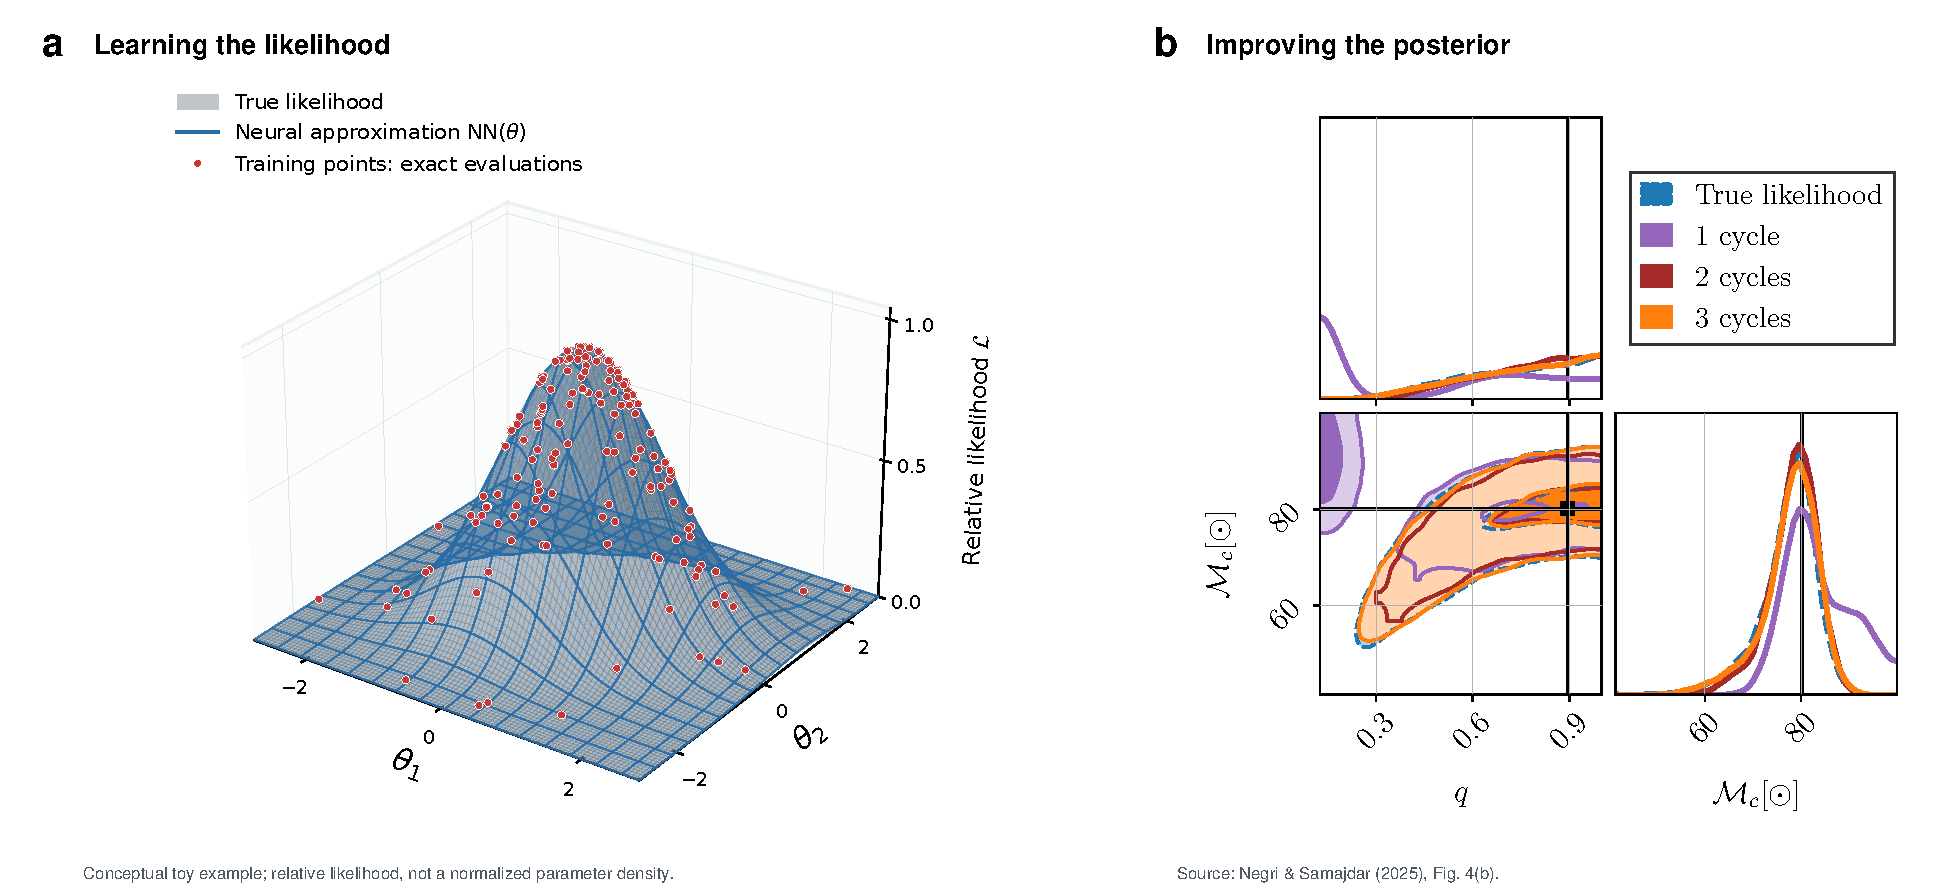
\includegraphics[width=\linewidth]{figures/nle_figure.pdf}
  \caption{\textbf{Learning and refining a likelihood approximation.}
    \textbf{a}, In a conceptual two-parameter example, training set consists of true likelihood evaluations
    (red dots) and constrain a neural network approximation (blue net surface) to a true
    likelihood surface (grey volume). Points of training set concentrate near the likelihood peak while also
    covering the outskirts; the height is relative likelihood. \textbf{b}, Successive training cycles improve posterior
    agreement with a reference analysis for parameters mass ratio and chirp mass.
    Subfigure b is reproduced from Fig.~4(b) of Negri and Samajdar.\cite{negri2025}}
  \label{fig:nle}
\end{figure}
% 图a为独立的概念示例，小型MLP实际拟合了玩具似然；不是FLEX数据或FLEX性能验证。
% 图b直接截自arXiv:2509.17606v1第7页；只裁剪并保留原坐标、曲线、图例。
% 图a的NN(theta)表示exp(f(theta))；示例网络在log-likelihood上训练。
% 红点参与了拟合，因此标为training points而非独立test set。

% P7.1 | 模拟验证 | 扩写后约90词
% 用频率解释可信区间覆盖率，例如标称90%的区间应在适当重复实验中表现出相应覆盖。
% 可选数字：99个模拟系统，总体P-P检验p约0.216；98/99在最多六轮内达到设定诊断阈值。
% 不用“所有参数均无偏”或“必然收敛到真实后验”；偏振角单项p约0.023尚待检查。
% 如篇幅不足，保留总体校准和迭代成功率，将异常简短放入P9。
% Simulated signals test whether the method preserves meaningful uncertainty
% estimates. The reported checks broadly support its calibration within the
% tested regime, while also identifying features that warrant closer investigation.

% P7.2 | 真实事件结果、速度与灵活性 | 扩写后约90词
% 聚焦GW150914同一IMRPhenomD波形下：pocomc原始似然656分钟，FLEX+pocomc40分钟。
% 这约为16倍总CPU时间加速；原始评估次数则从1.3e7降至1.8e5，约72倍。
% 不需要把两组数字都塞进成稿。选时间为主，避免模糊的“百倍更快”。
% 一句话说明不同波形及后续采样器上的演示；不能声称任何模型都已被验证。
% For GW150914, FLEX reproduces the main parameter constraints at substantially
% lower computational cost. Tests with several waveform models, together with
% reuse of the trained likelihood in another sampler, illustrate its practical flexibility.

% P7 | NLE在模拟信号与真实信号上的表现

Negri and Samajdar\cite{negri2025} first test their method on 99 simulated binary black hole signals. They check whether the inferred uncertainty ranges of parameters contained these known parameter values at the expected rates: a range assigned 90$\%$ probability should contain the true value in roughly 90$\%$ of the simulations. The overall agreement among all parameters supports the reliability of uncertainty estimates. They then analyze GW150914, a real signal from a black hole merger. Using the same waveform model, the neural likelihood recovers parameter distributions consistent with a conventional analysis while reducing the reported total CPU time, including training, from almost eleven hours to forty minutes. Analyses using four different waveform models also yield highly consistent source properties. These results demonstrate substantial computational savings within the range of signals tested.

% P8 | evidence与局限 | 扩写后约110词
% 解释似然代理还能用于估计evidence，但后验一致不自动保证evidence准确。
% 原文Table3中同模型log Z为286.1与285.2，差约0.9；可定性写仍有偏差需验证。
% 再用共同主线组织局限：重要区域是否充分覆盖。多峰、高SNR、更高维会增加困难。
% 当前是高质量双黑洞、对齐自旋并经边缘化的九维示范；更一般的进动/高阶模/校准尚需验证。
% 不罗列全部技术参数，也不要将“能更换模型后重新训练”写成“同一网络适用任何模型”。
% The likelihood surrogate also permits evidence calculations for comparing
% hypotheses, but agreement between posteriors does not by itself establish
% evidence accuracy. Multimodal distributions and more demanding signals remain
% important tests of the approach.

Neural likelihood estimator is successful in approximating posterior in simulations and GW150914, it features in being adaptable to various types of likelihood and keeping evidences like conventional Bayesian PE. Nevertheless it comes with limitations in many aspects. First is that the validation is implemented under simplified case of 9-parameter gravitational wave source. For example binaries whose spinning black holes carry non-parallel orbital and spin momentum would be more demanding in parameter dimensionality. Louder signals also weakens samplers' performance. Even the method in preparing training set is left for refinement in better approximating posterior.

% P9 | 收束与前景 | 扩写后约90词
% 回扣开头：降低成本可让研究者更充分地比较波形、噪声与物理假设。
% 可提作者提出的迁移学习，但标明是未来方向，不是已实现的跨事件复用。
% 仿照Spitz结尾，从具体工具提升到更广的科学收益，并留下需要验证的问题。
% 例如：更复杂、更精确的观测条件下，这种效率与可靠性的平衡能否维持？
% Cheaper inference could make repeated physical tests more accessible as
% gravitational-wave observations become richer. The next challenge is to retain
% this efficiency while demonstrating reliable uncertainties across a wider range
% of sources and analysis choices.

With further validation, cheaper inference by virtue of neural network could accelerate the examination of same events using a wider range of waveform models and physical assumptions on the fly. Such comparisons matter when researchers investigate how black hole binaries form or search for departures from general relativity. Agreement across analyses would strengthen confidence in these conclusions; disagreements could expose limitations in the models or even clues interpreted as new physics. Neural likelihood estimation could therefore help turn growing collections of signals into more thoroughly tested accounts of the systems that produced them.

\vspace{15pt}
\noindent{\large\bfseries AI Usage Statement}

AI tools are used in:
\begin{enumerate}
  \item Grammar and spelling check
  \item Illustration of Fig.\ref{fig:nle}
\end{enumerate}

\begin{thebibliography}{9}
  \small
  \bibitem{negri2025}
  Negri, L. \& Samajdar, A.
  Neural likelihood estimators for flexible gravitational wave data analysis.
  \href{https://arxiv.org/abs/2509.17606}{arXiv:2509.17606} (2025).

  \bibitem{veitch2015}
  Veitch, J. et al.
  Parameter estimation for compact binaries with ground-based gravitational-wave
  observations using the LALInference software library.
  \textit{Phys. Rev. D} \textbf{91}, 042003 (2015).
  \href{https://doi.org/10.1103/PhysRevD.91.042003}{doi:10.1103/PhysRevD.91.042003}.

  \bibitem{zackay2018}
  Zackay, B., Dai, L. \& Venumadhav, T.
  Relative Binning and Fast Likelihood Evaluation for Gravitational Wave Parameter Estimation.
  \href{https://arxiv.org/abs/1806.08792}{arXiv:1806.08792} (2018).

  \bibitem{dax2021}
  Dax, M. et al.
  Real-Time Gravitational Wave Science with Neural Posterior Estimation.
  \textit{Phys. Rev. Lett.} \textbf{127}, 241103 (2021).
  \href{https://doi.org/10.1103/PhysRevLett.127.241103}{doi:10.1103/PhysRevLett.127.241103}.

  \bibitem{dax2023}
  Dax, M. et al.
  Neural Importance Sampling for Rapid and Reliable Gravitational-Wave Inference.
  \textit{Phys. Rev. Lett.} \textbf{130}, 171403 (2023).
  \href{https://doi.org/10.1103/PhysRevLett.130.171403}{doi:10.1103/PhysRevLett.130.171403}.

  \bibitem{graff2012}
  Graff, P., Feroz, F., Hobson, M. P. \& Lasenby, A.
  BAMBI: blind accelerated multimodal Bayesian inference.
  \textit{Mon. Not. R. Astron. Soc.} \textbf{421}, 169--180 (2012).
  \href{https://doi.org/10.1111/j.1365-2966.2011.20288.x}{doi:10.1111/j.1365-2966.2011.20288.x}.
\end{thebibliography}
\end{document}
